\documentclass{article}[14pt]
\usepackage[T2A]{fontenc}
\usepackage{geometry}
\usepackage{fancyhdr}
\usepackage{tocloft}
\usepackage{hyperref}
\usepackage{titlesec}
\usepackage{graphicx}
\usepackage{caption}
\usepackage{wrapfig}
\usepackage[english, russian]{babel}
\geometry{
	a4paper,
	top=20mm, 
	right=25mm, 
	bottom=25mm, 
	left=25mm
}
\usepackage{amssymb}
\usepackage{fancyvrb}
\usepackage{fvextra}
\usepackage{ dsfont }
\usepackage{amsmath}
\usepackage{listings}
\usepackage{xcolor}
\usepackage{listingsutf8}
\usepackage{pdfpages}
\usepackage{lipsum}
\usepackage{makecell}
\usepackage{float}
\usepackage{longtable}


\lstset{ 
	basicstyle=\ttfamily\small,
	keywordstyle=\color{blue},
	inputencoding=utf8,              
	extendedchars=true,
	stringstyle=\color{red}
	commentstyle=\color{green},
	showspaces=false,         
	showstringspaces=false,  
	numbers=left,              
	numberstyle=\tiny\color{gray},
	breaklines=true,          
	frame=single,           
	captionpos=b,             
	tabsize=4,
	escapeinside={(*@}{@*)}, % для работы с нестандартными текстами
	literate={ё}{{\"o}}1 {Ё}{{\"O}}1 {«}{{\guillemotleft}}1 {»}{{\guillemotright}}1
	{А}{{\CYRA}}1 {Б}{{\CYRB}}1 {В}{{\CYRV}}1 {Г}{{\CYRG}}1 {Д}{{\CYRD}}1 
	{Е}{{\CYRE}}1 {Ж}{{\CYRZH}}1 {З}{{\CYRZ}}1 {И}{{\CYRI}}1 {Й}{{\CYRISHRT}}1 
	{К}{{\CYRK}}1 {Л}{{\CYRL}}1 {М}{{\CYRM}}1 {Н}{{\CYRN}}1 {О}{{\CYRO}}1 
	{П}{{\CYRP}}1 {Р}{{\CYRR}}1 {С}{{\CYRS}}1 {Т}{{\CYRT}}1 {У}{{\CYRU}}1 
	{Ф}{{\CYRF}}1 {Х}{{\CYRH}}1 {Ц}{{\CYRC}}1 {Ч}{{\CYRCH}}1 {Ш}{{\CYRSH}}1 
	{Щ}{{\CYRSHCH}}1 {Ъ}{{\CYRHRDSN}}1 {Ы}{{\CYRERY}}1 {Ь}{{\CYRSFTSN}}1 
	{Э}{{\CYREREV}}1 {Ю}{{\CYRYU}}1 {Я}{{\CYRYA}}1 
	{а}{{\cyra}}1 {б}{{\cyrb}}1 {в}{{\cyrv}}1 {г}{{\cyrg}}1 {д}{{\cyrd}}1 
	{е}{{\cyre}}1 {ж}{{\cyrzh}}1 {з}{{\cyrz}}1 {и}{{\cyri}}1 {й}{{\cyrishrt}}1 
	{к}{{\cyrk}}1 {л}{{\cyrl}}1 {м}{{\cyrm}}1 {н}{{\cyrn}}1 {о}{{\cyro}}1 
	{п}{{\cyrp}}1 {р}{{\cyrr}}1 {с}{{\cyrs}}1 {т}{{\cyrt}}1 {у}{{\cyru}}1 
	{ф}{{\cyrf}}1 {х}{{\cyrh}}1 {ц}{{\cyrc}}1 {ч}{{\cyrch}}1 {ш}{{\cyrsh}}1 
	{щ}{{\cyrshch}}1 {ъ}{{\cyrhrdsn}}1 {ы}{{\cyrery}}1 {ь}{{\cyrsftsn}}1 
	{э}{{\cyrerev}}1 {ю}{{\cyryu}}1 {я}{{\cyrya}}1               
}
\begin{document}
	
\thispagestyle{empty}
\begin{center}
	\Large {\bfseries МИНИСТЕРСТВО НАУКИ И ВЫСШЕГО ОБРАЗОВАНИЯ РОССИЙСКОЙ ФЕДЕРАЦИИ}
	\\
	\vspace{3mm}
	Федеральное государственное автономное образовательное учреждение высшего образования <<Санкт-Петербургский политехнический университет Петра Великого>>
	\\
	\vspace{3mm}
	Институт компьютерных наук и кибербезопасности
	\\
	\vspace{3mm}
	Высшая школа технологий искусственного интеллекта
	\\
	\vspace{3mm}
	Направление: 02.03.01 Математика и компьютерные науки
	\\
	\vspace{2cm}
	\large{
		Методы тестирования программного обеспечения}
	\\
	\LARGE{
		Отчет по лабораторной работе №1\\
		<<Инспекция кода>>}
\end{center}

\vspace{5.5cm}
\begin{flushleft}
	\Large
	Студент
	\\
	группы 5130201/30101
	\\
	\vspace{2cm}
	\Large
	Преподаватель
	\\ 
\end{flushleft}
\vspace{-4.6cm}
\begin{flushright}
	\Large
	\line(1,0){2cm}
	\hspace{0.4cm}
	Шишмаков В.О.
	\\
	\vspace{2,7cm}
	\hspace{2cm}
	\Large
	\line(1,0){2cm}
	\hspace{0.4cm}
	Курочкин М. А.
	\hspace{-0.1cm}
	
\end{flushright}

\vspace{1cm}
\hspace{9.8cm}
{
	\Large
	\vspace{0.8cm}
	<<\underline{\hspace{1cm}}>>\underline{\hspace{2.5cm}} 2026 г.
}
\hfill \break
\hfill \break
\hfill \break
\hfill \break
\begin{center} \large{Санкт-Петербург, 2026} \end{center}
\pagebreak

\titleformat{\section}
{\Huge\bfseries}
{\thesection\;}
{0.65cm}
{}
\titleformat{\subsection}
{\huge\bfseries}
{\thesubsection\;}
{0.65cm}
{}
\titleformat{\subsubsection}
{\Large\bfseries}
{\thesubsubsection\;}
{0.65cm}
{}
\titlespacing*{\section}
{0em}
{1.5ex plus 1ex minus 0.2ex}
{1.5ex plus 1ex minus 0.2ex}	

\renewcommand*\contentsname{\huge{Содержание}}
\Large{
	\tableofcontents}
\pagebreak

\section*{Введение}
\addcontentsline{toc}{section}{Введение}

В данной работе рассматривается применение одного из подходов к ручному тестированию, а именно —-- инспекция программного кода.

Под тестированием понимается процесс запуска программы с целью выявления дефектов.

Долгое время среди разработчиков преобладало мнение, что код создается исключительно для выполнения машиной и не рассчитан 
на восприятие человеком, в связи с чем единственным способом его проверки считался прогон на компьютере. Ситуация начала 
изменяться в начале 1970-х годов благодаря инициативе специалистов, которые первыми осознали значимость анализа кода как 
важной составляющей процессов тестирования и отладки.

Эффективность применения такой проверки зависит от целого ряда условий: размер и сложность разрабатываемой системы, 
количество участников команды, плотность графика работ (например, является ли он сжатым или относительно свободным), 
а также уровень подготовки и профессиональные привычки коллектива разработчиков.

Рассмотрим подход к тестированию, который выполняется человеком и не требует применения вычислительной техники —-- так 
называемое ручное тестирование. Данный подход доказал свою результативность при поиске неисправностей, и его варианты 
стоит внедрять в каждом проекте по созданию программ. Методы ручного контроля необходимо использовать для проверки исходного 
кода ещё до этапа его прогона на компьютере. Кроме того, допустимо разрабатывать собственные аналогичные приемы и внедрять 
их на более ранних этапах разработки (к примеру, после завершения отдельных фаз проектирования).

Во-первых, общеизвестно, что выявление дефектов на ранних стадиях существенно удешевляет их исправление и повышает шансы 
на то, что внесенные правки окажутся верными. Во-вторых, было подмечено, что у разработчика, проверяющего программу на 
компьютере, постепенно меняется психологическое состояние. У него нарастает эмоциональное напряжение и появляется острое 
стремление побыстрее избавиться от надоевшей ошибки. Вследствие этого при устранении неполадок, найденных во время 
компьютерного тестирования, программист совершает больше промахов по сравнению с исправлением дефектов, обнаруженных ранее.

Еще одним плюсом сквозного анализа, способствующим уменьшению затрат на отладку, выступает возможность четко определить 
местонахождение ошибки. Более того, при тщательной проверке кода зачастую удается найти сразу несколько ошибок, которые 
затем можно исправить комплексно. При тестировании же на компьютере чаще всего наблюдаются лишь последствия сбоев 
(например, программа зависает или выдает некорректные данные), а сами ошибки выявляются и исправляются поочередно.

\pagebreak

\section{Постановка задачи}

В ходе выполнения этой лабораторной работы необходимо выполнить инспекцию программного кода, 
действуя от лица разработчика приложения.

\noindent \textbf{Задачи:}

\begin{itemize}
    \item ознакомиться с подходами к ручному тестированию;
    \item осуществить проверку кода;
    \item оценить итоги проведенного тестирования;
    \item внести правки в программу согласно замечаниям тестировщика.
\end{itemize}

\pagebreak

\section{Методы ручного тестирования}

\subsection{Инспекция кода}

\textbf{Инспекция кода} --- комплекс процедур и приемов, направленных на выявление дефектов путем коллективного разбора 
(чтения) исходного текста. Чаще всего, когда речь заходит об инспекциях, основной упор делается на организационные моменты, 
оформление документации и тому подобные аспекты.

\bigskip

\noindent \textbf{Состав команды для инспекции кода}

Как правило, в команду входит четыре человека, один из которых выполняет функции модератора. На эту роль 
назначается опытный программист, не являющийся автором рассматриваемого кода, при этом глубокое знание проверяемой 
программы от него не требуется. В его задачи входит:

\begin{itemize}
    \item подготовка и рассылка материалов членам группы, а также составление регламента встречи;
    \item ведение заседания;
    \item фиксация всех выявленных недочетов;
    \item последующий контроль за тем, чтобы найденные проблемы были исправлены.
\end{itemize}

Второй участник —-- это непосредственно разработчик программы. Остальные два члена команды —-- проектировщик системы 
и тестировщик. Последний должен не только разбираться в методиках проверки ПО, но и знать типичные ошибки, о чем пойдет 
речь далее.

\bigskip

\noindent \textbf{Порядок организации инспекционных встреч}

За несколько суток до назначенного сбора модератор обеспечивает всех участников распечатками кода и техническим 
заданием на проект. Это необходимо, чтобы к началу встречи каждый успел изучить предоставленные материалы. 
Само заседание строится по следующему плану.

\begin{enumerate}
    \item Разработчик поясняет логику функционирования программы, последовательно проходя по каждому оператору. 
    В процессе объяснения остальные члены команды должны задавать ему уточняющие вопросы, помогающие выявить 
    потенциальные проблемы. Нередко часть недочетов находит сам программист во время рассказа, а не другие участники. 
    Таким образом, простое проговаривание кода вслух при публичном описании его работы оказывается действенным способом 
    поиска ошибок.

    \item Члены группы исследуют текст программы, опираясь на подготовленные на основе предыдущего опыта перечни 
    характерных ошибок.
\end{enumerate}

Задача модератора —-- поддерживать обсуждение в продуктивном ключе и следить, чтобы участники сосредоточились 
именно на поиске дефектов, а не на их исправлении. Доработка кода производится разработчиком после завершения встречи.

После завершения встречи разработчику передается перечень выявленных недочетов. Если этот перечень оказывается объемным 
либо исправление проблем требует серьезной переработки программы, ведущий может назначить повторную инспекцию после того, 
как все ошибки будут устранены. Полученный список анализируется, и после классификации ошибок он пополняет существующий 
каталог типичных дефектов, что способствует росту эффективности будущих проверок кода. Как уже упоминалось, 
цель инспекции —-- найти ошибки, а не исправить их. Однако, если обнаруженная проблема не представляет большой сложности, 
группа может принять решение о том, чтобы двое-трое участников, включая автора кода, подготовили варианты корректировки 
проекта. Обсуждение этих предложений, в свою очередь, позволяет детальнее сфокусироваться на соответствующей части проекта. 
В ходе дискуссии о возможных изменениях кто-либо из участников может выявить еще одну проблему.

Теперь, когда перед группой стоят уже две задачи, связанные с одним и тем же фрагментом проекта, обсуждение становится 
более активным, и его участники активно делятся своими идеями. Благодаря такому подходу на углубленный анализ данного 
участка и обнаружение сопутствующих проблем может уйти всего несколько минут.

\bigskip

\noindent \textbf{Дополнительные преимущества инспекционного подхода}

Помимо своей главной функции (содействия в поиске дефектов) инспектирование кода дает и ряд других положительных 
результатов. В частности, разработчик получает возможность услышать объективную оценку своего стиля написания программ, 
использованных алгоритмов и методов проверки. Другие члены команды, изучая ошибки и подходы к программированию коллег, 
также обогащают свой профессиональный опыт.

\bigskip

\noindent \textbf{Контрольные списки возможных ошибок для инспекций}

\begin{figure}[H]
    \centering
    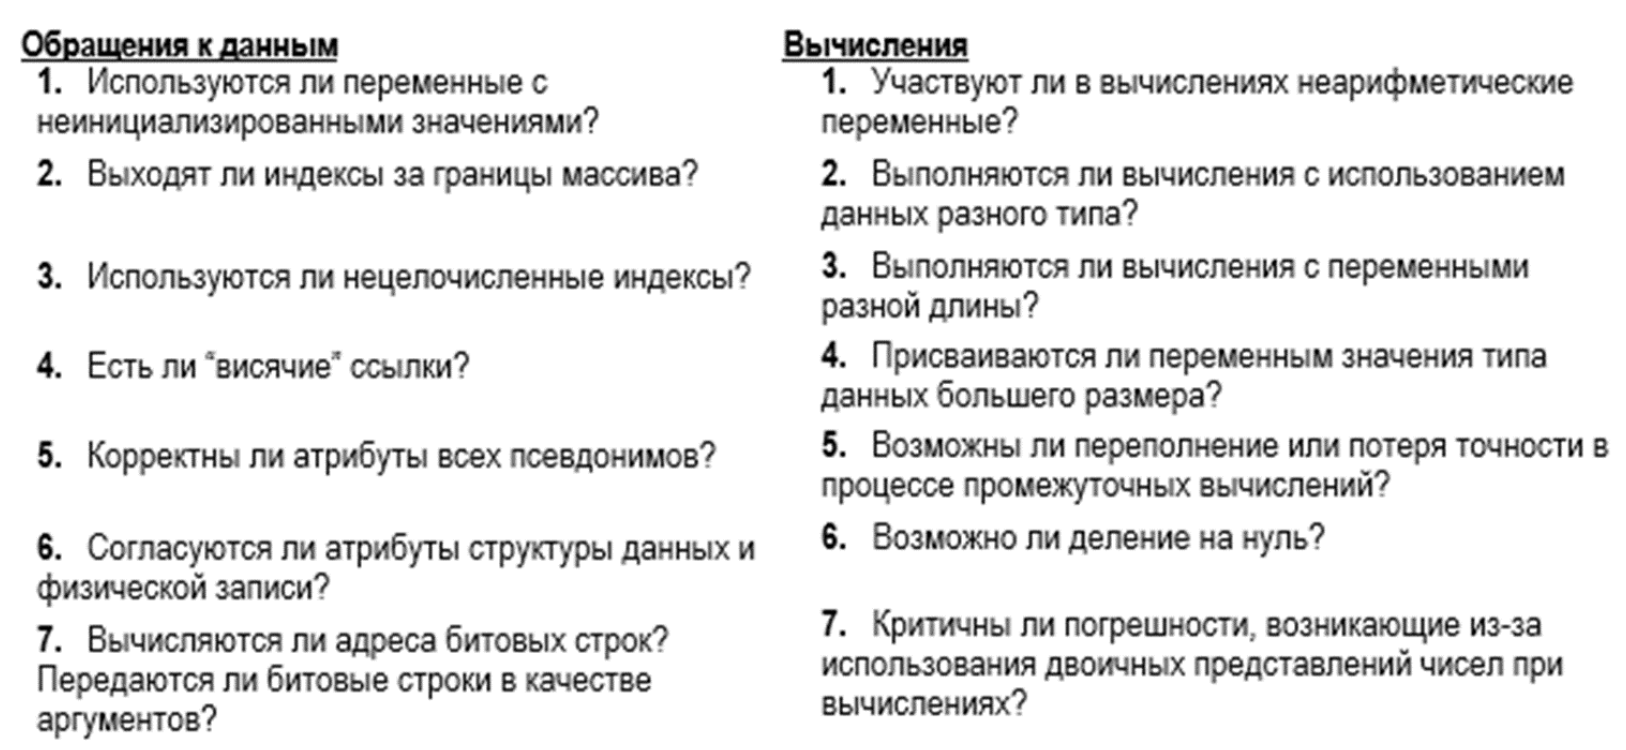
\includegraphics[width=\textwidth]{questions1.png}
\end{figure}

\begin{figure}[H]
    \centering
    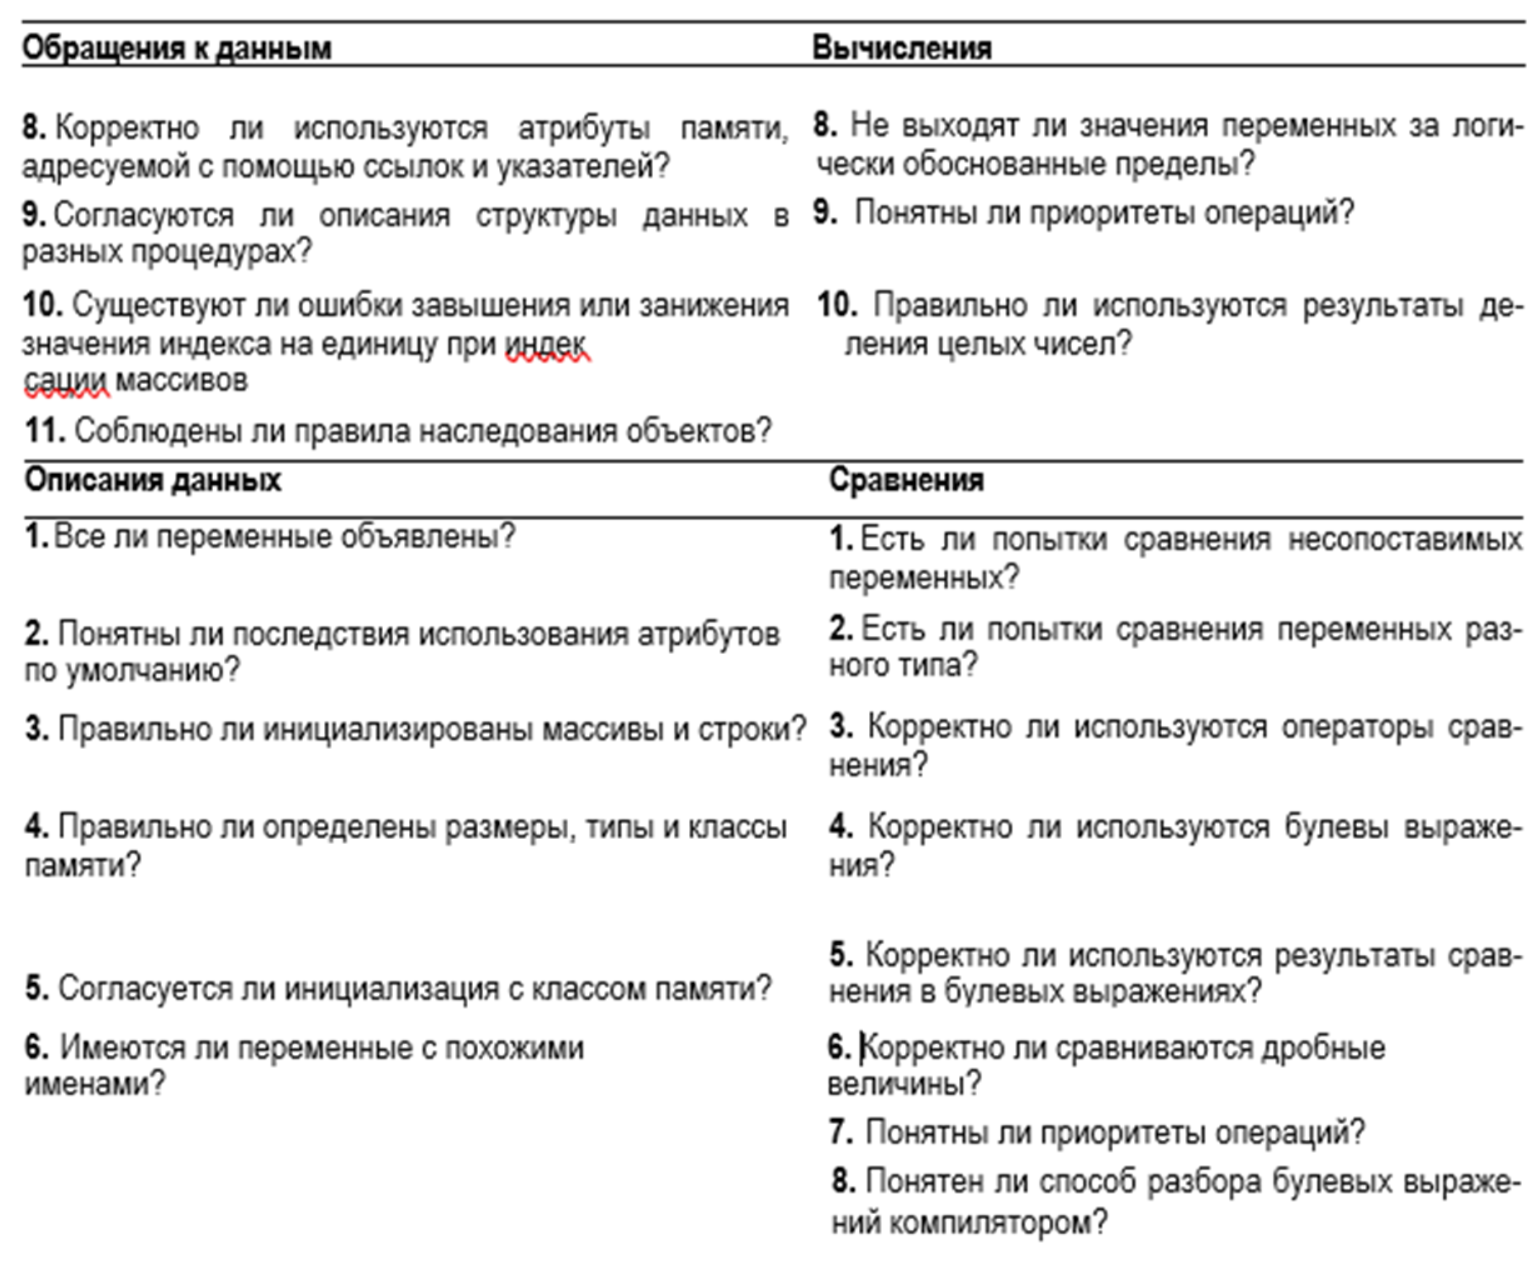
\includegraphics[width=\textwidth]{questions2.png}
\end{figure}

\begin{figure}[H]
    \centering
    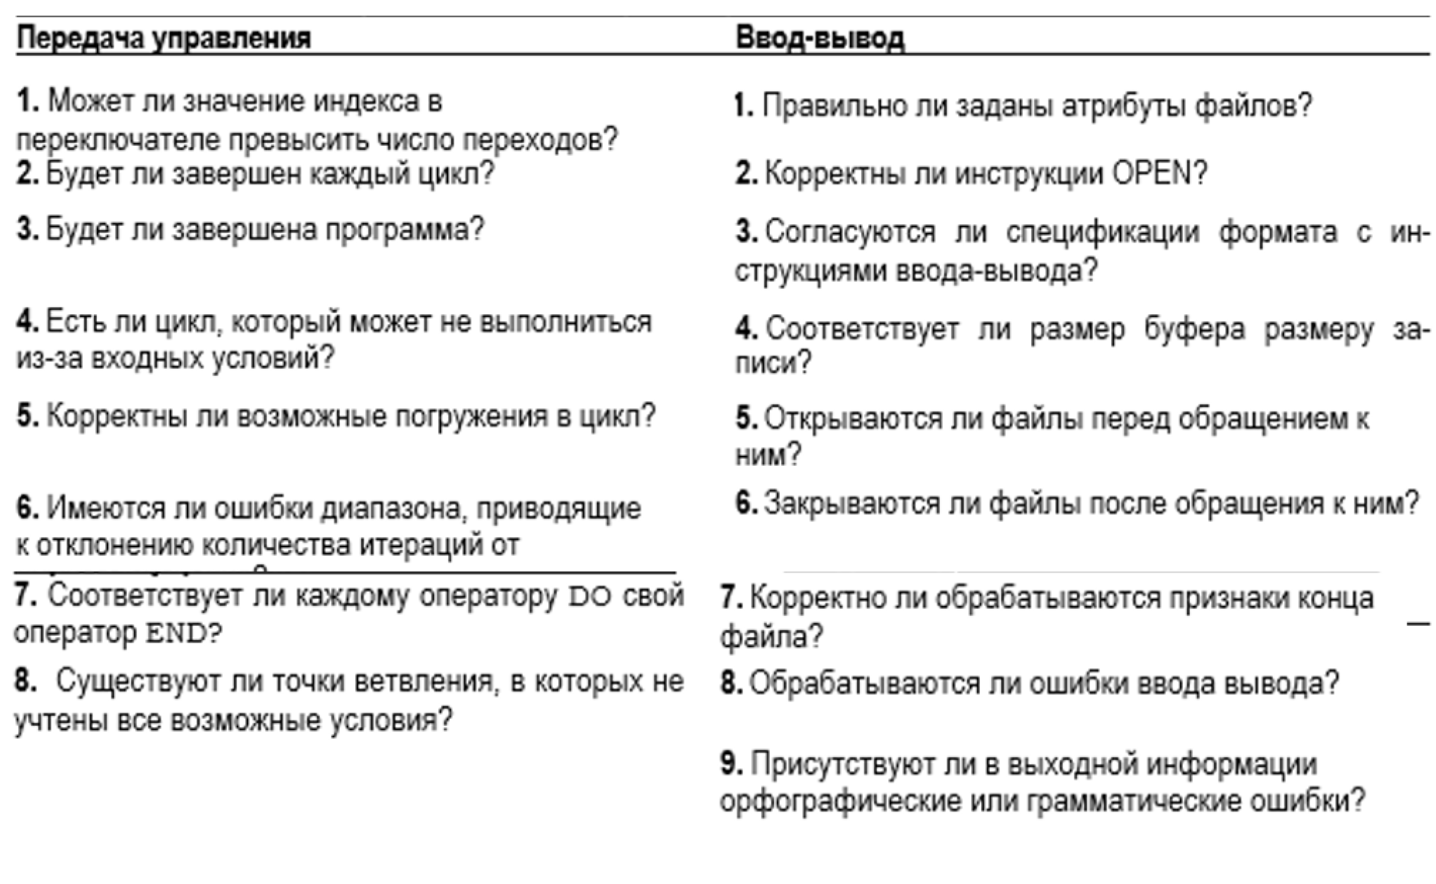
\includegraphics[width=\textwidth]{questions3.png}
\end{figure}

\begin{figure}[H]
    \centering
    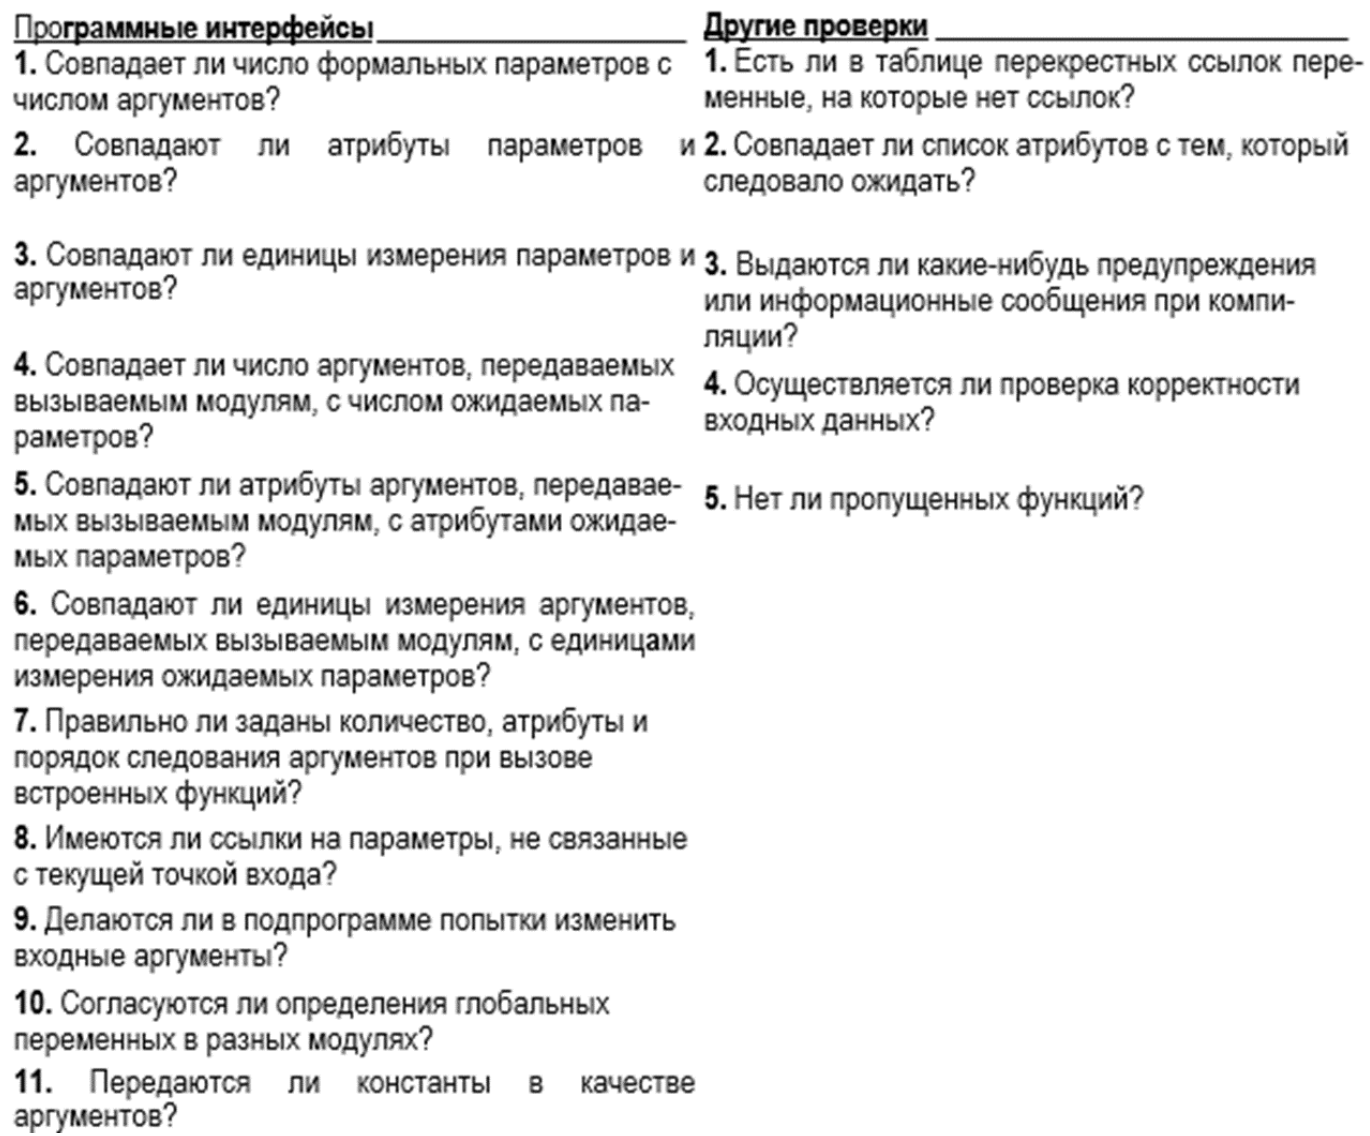
\includegraphics[width=\textwidth]{questions4.png}
\end{figure}

\subsection{Сквозные просмотры}

Подобно инспекции, сквозной анализ кода представляет собой комплекс процедур и приемов, направленных на выявление дефектов 
в программе путем ее коллективного изучения членами проверяющей команды. Данный метод во многом схож с процессом 
инспектирования, однако использует несколько иные организационные подходы и техники.

Как и при инспекции, сквозная проверка организуется в виде непрерывного совещания, продолжительность которого не 
превышает двух часов. Количество участников команды, задействованных в сквозном анализе, составляет от трех до пяти человек. 
Один из них выполняет обязанности, схожие с ролью модератора в инспекционной группе. Другой участник выступает в роли 
секретаря, фиксирующего все обнаруженные недочеты. Третий —-- это тестировщик. Мнения относительно того, кто именно должен 
входить в состав группы и стоит ли расширять ее до пяти человек, различаются. Безусловно, одним из этих людей обязан быть 
разработчик, создавший программу. Среди других возможных кандидатов можно назвать:

\begin{itemize}
    \item специалиста по языку программирования, на котором написан код;
    \item неопытного программиста (взгляд которого еще не сформирован предыдущей практикой);
    \item сотрудника, который в дальнейшем будет сопровождать данную программу;
    \item представителя другого проекта;
    \item коллегу автора программы из той же команды разработчиков.
\end{itemize}

Процедура проведения сквозного просмотра стартует аналогично инспекции: за несколько дней до встречи участникам 
раздаются необходимые материалы, чтобы у них была возможность предварительно изучить проверяемое программное обеспечение. 
Однако само заседание строится по-другому. Вместо последовательного чтения кода или его сверки с перечнем типичных ошибок, 
члены группы «имитируют работу компьютера». Участник, выполняющий роль тестировщика, приносит на совещание заранее 
подготовленные на бумаге тесты —-- характерные наборы входных данных для программы или ее модуля. 
В ходе встречи присутствующие мысленно «прогоняют» каждый тест, то есть вручную обрабатывают тестовые данные, следуя логике 
программы. Текущее состояние программы фиксируется на бумаге или на доске.

Разумеется, количество тестов не должно быть большим, и они обязаны быть несложными, поскольку скорость ручного выполнения 
операций несопоставимо ниже, чем машинные вычисления. Таким образом, сами тесты не являются самоцелью; скорее, они выступают 
инструментом для вовлечения участников в процесс и основой для обсуждения с разработчиком вопросов, связанных с логикой 
построения программы и сделанными допущениями. В ходе большинства сквозных проверок непосредственно при выполнении тестов 
выявляется меньше ошибок, чем в процессе опроса программиста.

\subsection{Проверка за столом}

Третий подход к ручному выявлению дефектов — это хорошо известный метод «настольной проверки» (или «ручной прогонки»). 
Его можно рассматривать как инспекцию либо сквозной анализ, выполняемые единолично: человек самостоятельно изучает код, 
сверяет его с перечнем типичных ошибок и (или) мысленно пропускает через логику программы тестовые данные.

Для большинства специалистов настольная проверка оказывается сравнительно малопродуктивной. Это связано прежде всего с тем, 
что данный процесс практически не структурирован. Вторая, более существенная причина заключается в том, что такой подход 
противоречит одному из базовых принципов тестирования, согласно которому проверка разработчиком собственного кода, 
как правило, малоэффективна. Поэтому оптимальным решением было бы поручать эту проверку другому лицу, 
однако даже в таком варианте результативность будет ниже, чем при коллективных инспекциях или сквозных просмотрах. 
Именно по этой причине предпочтительнее проводить сквозные проверки или инспекции в группе.

Коллективный формат с обсуждением способствует возникновению духа здорового соперничества, так как каждый участник стремится 
проявить себя при поиске ошибок. При настольной проверке этот, безусловно, ценный эффект отсутствует. Одним словом, 
«ручной прогон» приносит определенную пользу, однако его эффективность значительно уступает инспекциям и сквозным анализам 
кода.

\subsection{Рецензирование}

Последний из рассматриваемых подходов к экспертному анализу программ человеком не относится напрямую к тестированию ПО 
(то есть его цель —-- не поиск дефектов). Тем не менее, его описание приводится здесь, поскольку он основан на идее чтения и 
оценки программного кода.

Рецензирование представляет собой процедуру, при которой анонимно оцениваются общие показатели качества программы, 
такие как удобство сопровождения, возможность расширения, простота использования и понятность кода.

Задача этого метода —-- дать разработчику возможность получить независимую оценку своей работы.

Общую координацию процесса осуществляет администратор, назначаемый из числа программистов. Администратор, в свою очередь, 
формирует группу рецензентов численностью от 6 до 20 человек (6 — это минимальное количество, необходимое для сохранения 
анонимности оценок). Предполагается, что все участники работают в одной области.

Каждый из участников предоставляет для рецензирования две свои программы: одну, которую он считает своей лучшей работой, 
и другую, которую он оценивает как наихудшую с точки зрения качества.

После сбора всех программ они случайным образом распределяются между участниками. Каждому рецензенту достается для 
оценки четыре программы: две из категории «лучших» и две из категории «худших», однако принадлежность к той или иной 
категории не разглашается. На изучение одной программы отводится 30 минут, после чего заполняется оценочная форма. 
Завершив просмотр всех четырех программ, рецензент сравнивает их между собой по качеству. В анкете предлагается оценивать 
программы по десятибалльной шкале (где «1» означает однозначное «да», а «10» — столь же определенное «нет»), отвечая, к 
примеру, на следующие вопросы.

\begin{itemize}
    \item Легко ли было разобраться в программе?
    \item Хорошо ли различимы и достаточно ли разумны используемые в программе
    концепции высокоуровневого проектирования?
    \item Хорошо ли различимы и достаточно ли разумны используемые в программе
    концепции низкоуровневого проектирования?
    \item Легко ли вам было бы модифицировать данную программу?
    \item Испытывали бы вы чувство удовлетворения, написав такую программу?
\end{itemize}

Рецензенту также предлагается сформулировать свои замечания по программе и предложения по её усовершенствованию. 
После того как все программы будут оценены, каждому автору передаются заполненные анкеты на его две работы. Дополнительно 
участникам предоставляется статистическая сводка, содержащая как обобщенные, так и детальные сведения о месте их программ 
в общем рейтинге, а также анализ того, насколько выставленные ими оценки чужим программам совпадают с мнением других 
рецензентов.

\pagebreak

\section{Описание тестируемой программы}

\noindent \textbf{Название:} Реализация длинной арифметики для целых чисел.

    \noindent \textbf{Дано:}

    \begin{itemize}
        \item $M$ --- целое число разрядов.
        \item $N$ --- целое число, характеризующее систему счисления.
        \item $a, b$ --- числа, над которыми производятся операции.
    \end{itemize}

    \noindent \textbf{Требуется:} Реализовать операции сложения, вычитания, умножения и целочисленного деления над целыми числами.

    \noindent \textbf{Ограничения:}

    \begin{itemize}
        \item $N > 0$
        \item $M > 0$
        \item $a \geq 0$
        \item $b \geq 0$
    \end{itemize}
    
    \subsection{Спецификация}

    {\large{
    \begin{longtable}{|p{0.3cm}|p{3cm}|p{5cm}|p{6cm}|}
    \hline
    \textbf{№} & \textbf{Вход} & \textbf{Выход} & \textbf{Реакция программы} \\ \hline
    1 & $a = 15000000000; b = 1000000000; M = 10; N = 2$ & a = [0, 0] --- 0;
b = [0, 0] --- 0;
Sum: [0, 0] --- 0;
Sub: [0, 0] --- 0;
Mul: [0, 0] --- 0;
Div: [0] --- 0; & Программа принимает на вход числа a и b приводит их в формат длинной 
арифметики и выполняет над ними 4 операции. Выводит числа a и b, а также результаты операций над ними \\ \hline
    2 & $a = 2441; b = 2111; M = 10; N = 2$ & a = [4, 1] --- 41;
b = [1, 1] --- 11;
Sum: [5, 2] --- 52;
Sub: [3, 0] --- 30;
Mul: [5, 1] --- 51;
Div: [0, 3] --- 3; & Программа принимает на вход числа a и b приводит их в формат длинной 
арифметики и выполняет над ними 4 операции. Выводит числа a и b, а также результаты операций над ними \\ \hline
    3 & $a = 2441; b = 0; M = 10; N = 2$ & a = [4, 1] --- 41;
b = [0, 0] --- 0;
Sum: [4, 1] --- 41;
Sub: [4, 1] --- 41;
Mul: [0, 0] --- 0;
Div: [0] --- 0; & Программа принимает на вход числа a и b приводит их в формат длинной 
арифметики и выполняет над ними 4 операции. Выводит числа a и b, а также результаты операций над ними \\ \hline
    \end{longtable}}}

\subsection{Исходный код}

Исходный код программы на языке программирования Python представлен в листинге \ref{lst:code}.

\begin{lstlisting}[caption={Исходный код программы}, label=lst:code]
M = 10
N = 2


def normalize(num, M=None, N=None):
    while len(num) > 1 and num[0] == 0:
        num = num[1:]
    return num


def to_int(num, M):
    num = normalize(num)
    result = 0
    for digit in num:
        result = result * M + digit
    return result


def from_int(num, M, N):

    mod = M ** N
    num %= mod

    digits = []
    for _ in range(N):
        digits.append(num % M)
        num //= M
    digits.reverse()
    return digits  


def compare(first_value, second_value):
    a = normalize(first_value[:])
    b = normalize(second_value[:])
    if len(a) > len(b):
        return 1
    if len(a) < len(b):
        return -1
    for x, y in zip(a, b):
        if x > y:
            return 1
        if x < y:
            return -1
    return 0


def sum(first_value, second_value, M, N):
    a = first_value[-N:]
    b = second_value[-N:]
    max_len = max(len(a), len(b))
    a = [0] * (max_len - len(a)) + a
    b = [0] * (max_len - len(b)) + b

    carry = 0
    res = [0] * (max_len + 1)
    for i in range(max_len - 1, -1, -1):
        s = a[i] + b[i] + carry
        res[i + 1] = s % M
        carry = s // M
    res[0] = carry

    res = res[-N:]
    return res


def sub(first_value, second_value, M, N):
    a = first_value[-N:]
    b = second_value[-N:]
    max_len = max(len(a), len(b))
    a = [0] * (max_len - len(a)) + a
    b = [0] * (max_len - len(b)) + b

    res = [0] * max_len
    borrow = 0
    for i in range(max_len - 1, -1, -1):
        val = a[i] - b[i] - borrow
        if val < 0:
            val += M
            borrow = 1
        else:
            borrow = 0
        res[i] = val

    if borrow == 1:
        add_back = [M - 1] * max_len
        carry = 1
        for i in range(max_len - 1, -1, -1):
            val = res[i] + add_back[i] + carry
            res[i] = val % M
            carry = val // M

    res = res[-N:]
    return res


def mul_small(a, k, M, N):
    if k == 0 or a == [0]:
        return [0] * N

    a = a[-N:]
    res = [0] * (len(a) + 1)
    carry = 0
    for i in range(len(a) - 1, -1, -1):
        prod = a[i] * k + carry
        res[i + 1] = prod % M
        carry = prod // M
    res[0] = carry

    res = res[-N:]
    return res


def times(first_value, second_value, M, N):
    a = first_value[-N:]
    b = second_value[-N:]
    if a == [0] * len(a) or b == [0] * len(b):
        return [0] * N

    res = [0] * (2 * N)
    len_a = len(a)
    len_b = len(b)

    for i in range(len_a - 1, -1, -1):
        carry = 0
        for j in range(len_b - 1, -1, -1):
            idx = i + j + 1
            total = res[idx] + a[i] * b[j] + carry
            res[idx] = total % M
            carry = total // M
        res[i] += carry

    res = res[-N:]
    return res


def div(first_value, second_value, M, N):
    if compare(second_value, [0]) == 0:
        return [0] # division by zero

    a = first_value[-N:]
    b = second_value[-N:]
    a = normalize(a)
    b = normalize(b)
    if compare(a, b) < 0:
        return [0] * N

    quotient = []
    remainder = [0]
    for digit in a:
        
        remainder = remainder + [digit]
        remainder = normalize(remainder)

        lo, hi = 0, M - 1
        q = 0
        while lo <= hi:
            mid = (lo + hi) // 2
            prod = mul_small(b, mid, M, N)
            if compare(prod, remainder) <= 0:
                q = mid
                lo = mid + 1
            else:
                hi = mid - 1
        quotient.append(q)
        if q:
            remainder = sub(remainder, mul_small(b, q, M, N), M, N)

    quotient = quotient[-N:]
    return quotient


a = from_int(2441, M, N)  
b = from_int(0, M, N)   

print(f"a = {a} --- {to_int(a, M)}")
print(f"b = {b} --- {to_int(b, M)}")

print("Sum:", sum(a, b, M, N), "---", to_int(sum(a, b, M, N), M))
print("Sub:", sub(a, b, M, N), "---", to_int(sub(a, b, M, N), M))
print("Mul:", times(a, b, M, N), "---", to_int(times(a, b, M, N), M))
print("Div:", div(a, b, M, N), "---", to_int(div(a, b, M, N), M))
\end{lstlisting}

\pagebreak

\section{Описание проведенной инспекции кода}

\noindent \textbf{Группа испекции кода:}

\begin{itemize}
	\item Программист (разработчик программы): Шишмаков Владимир.
	
	\item Специалист по тестированию: Чурова Софья.
\end{itemize}

В начале встречи была изложена логика работы программы, а также предоставлена её спецификацию и ограничения. 
В ходе инспекции было задано 53 вопроса, направленных на выявление расхождений с требованиями спецификации.

Я, как программист-разработчик, ответил на все вопросы и получил обратную связь от тестировщика. После чего был составлен 
протокол заседания, в котором зафиксированы заданные вопросы и данные на них ответы, а также рекомендации по 
устранению обнаруженных несоответствий.

\subsection{Протокол заседания}

\begin{enumerate}

\item \textbf{Используются ли переменные с неинициализированными значениями?}
\\
Нет. Все переменные в функциях либо получают значения через параметры, либо инициализируются явно.

\item \textbf{Выходят ли индексы за границы массива?}
\\
Потенциально, да. В функции \texttt{times} при обращении к \texttt{res[idx]} для \texttt{idx = i + j + 1} возможно попадание в уже существующий диапазон, но индекс \texttt{i + j + 1} может быть близок к границе, если \texttt{i} и \texttt{j} максимальны. Однако резервируется массив длиной \(2N\), что должно быть достаточно для произведения двух N-разрядных чисел. Но код не содержит явных проверок на допустимость индексов.

\item \textbf{Используются ли нецелочисленные индексы?}
\\
Нет. Все индексы — целые числа.

\item \textbf{Есть ли <<висячие>> ссылки?}
\\
В Python нет классических <<висячих>> ссылок благодаря сборщику мусора. Однако есть ситуации, когда переменная ссылается на объект, который больше не нужен, но это не приводит к ошибкам.

\item \textbf{Корректны ли атрибуты всех псевдонимов?}
\\
В коде используются присваивания списков, что создает новый список, а не псевдоним, поэтому атрибуты не нарушаются.

\item \textbf{Согласуются ли атрибуты структуры данных и физической записи?}
\\
Да, структура данных (список цифр) полностью соответствует логике длинной арифметики, где каждый элемент — цифра в системе с основанием M.

\item \textbf{Вычисляются ли адреса битовых строк? Передаются ли битовые строки в качестве аргументов?}
\\
Нет, битовые строки не используются.

\item \textbf{Корректно ли используются атрибуты памяти, адресуемой с помощью ссылок и указателей?}
\\
В Python все переменные являются ссылками на объекты. Функции вроде \texttt{normalize} возвращают новый список, не модифицируя исходный, что безопасно. Однако \texttt{normalize} объявлена как принимающая \texttt{M} и \texttt{N}, но не использует их, что избыточно.

\item \textbf{Согласуются ли описания структуры данных в разных процедурах?}
\\
Да, все функции ожидают список цифр и параметры \texttt{M}, \texttt{N}, что согласовано.

\item \textbf{Существуют ли ошибки завышения или занижения значения индекса на единицу при индексации массивов?}
\\
В функции \texttt{sum} используется \texttt{res[i + 1] = s \% M}, что корректно. В \texttt{times} при \texttt{idx = i + j + 1} также все верно. Однако в \texttt{div} есть потенциальная ошибка: \texttt{remainder = remainder + [digit]} может привести к тому, что \texttt{remainder} станет длиннее ожидаемого, но индексация внутри не вызывает проблем.

\item \textbf{Участвуют ли в вычислениях неарифметические переменные?}
\\
Нет, все переменные либо целые числа, либо списки целых чисел.

\item \textbf{Выполняются ли вычисления с использованием данных разного типа?}
\\
Нет. Все арифметические операции производятся над целыми числами.

\item \textbf{Выполняются ли вычисления с переменными разной длины?}
\\
В длинной арифметике это неизбежно. Например, при сложении числа выравниваются по длине, что корректно обрабатывается.

\item \textbf{Присваиваются ли переменным значения типа данных большего размера?}
\\
В Python динамическая типизация, и размер чисел не ограничен, поэтому данная проблема отсутствует.

\item \textbf{Возможны ли переполнение или потеря точности в процессе промежуточных вычислений?}
\\
Нет, поскольку Python поддерживает целые числа произвольной точности. Промежуточные результаты вроде \texttt{a[i] * b[j] + carry} могут быть большими, но это допустимо.

\item \textbf{Возможно ли деление на нуль?}
\\
Да, это возможно. В функции \texttt{div} есть проверка: \texttt{if compare(second\_value, [0]) == 0: return [0]}. Формально деление на ноль перехватывается, но возврат \texttt{[0]} логически неверно.

\item \textbf{Критичны ли погрешности, возникающие из-за использования двоичных представлений чисел при вычислениях?}
\\
Нет, так как работа идет с целыми числами и заданной системой счисления. Двоичное представление Python не влияет на точность целочисленных операций.

\item \textbf{Не выходят ли значения переменных за логически обоснованные пределы?}
\\
Входные числа могут быть любыми, но внутри они обрезаются до N разрядов через взятие последних N элементов (\texttt{[-N:]}). Это может привести к потере значимых разрядов, что является логической ошибкой.

\item \textbf{Понятны ли приоритеты операций?}
\\
Да, выражения просты и используют скобки для явного указания порядка.

\item \textbf{Правильно ли используются результаты деления целых чисел?}
\\
В функции \texttt{div} для подбора цифры частного используется целочисленное деление в бинарном поиске, что корректно. В остальных местах целочисленное деление применяется для вычисления переноса (\texttt{carry = s // M}) — это верно.

\item \textbf{Все ли переменные объявлены?}
\\
В Python переменные не требуют предварительного объявления, но все используемые имена определены до использования.

\item \textbf{Понятны ли последствия использования атрибутов по умолчанию?}
\\
Глобальные переменные \texttt{M} и \texttt{N} используются во всех функциях, хотя передаются как аргументы. Это может привести к путанице, если функции будут вызываться с другими значениями.

\item \textbf{Правильно ли инициализированы массивы и строки?}
\\
Да, все списки инициализируются явно (например, \texttt{res = [0] * max\_len}).

\item \textbf{Правильно ли определены размеры, типы и классы памяти?}
\\
Для Python это неактуально, но логически размеры списков соответствуют ожидаемым.

\item \textbf{Согласуется ли инициализация с классом памяти?}
\\
В Python все переменные хранятся в куче, инициализация корректна.

\item \textbf{Имеются ли переменные с похожими именами?}
\\
Внутри функций параметры называются \texttt{first\_value}, \texttt{second\_value}, а локальные переменные — \texttt{a}, \texttt{b}. Это не приводит к конфликтам, но может вызывать путаницу при чтении кода.

\item \textbf{Есть ли попытки сравнения несопоставимых переменных?}
\\
Нет, сравниваются только списки цифр с помощью функции \texttt{compare}, которая корректно обрабатывает списки.

\item \textbf{Есть ли попытки сравнения переменных разного типа?}
\\
Нет, все сравнения происходят между списками или между целыми числами.

\item \textbf{Корректно ли используются операторы сравнения?}
\\
В коде не используются напрямую операторы \texttt{<}, \texttt{>} для списков — вместо этого вызывается \texttt{compare}, что правильно.

\item \textbf{Корректно ли используются булевы выражения?}
\\
Да, например, в цикле \texttt{while lo <= hi:} условие корректно.

\item \textbf{Корректно ли используются результаты сравнения в булевых выражениях?}
\\
Да, возвращаемые значения \texttt{compare} (-1, 0, 1) используются в условных операторах правильно.

\item \textbf{Понятны ли приоритеты операций?}
\\
Да, выражения просты и используют скобки.

\item \textbf{Понятен ли способ разбора булевых выражений композитором?}
\\
Для Python это не проблема — интерпретатор четко следует правилам приоритета.

\item \textbf{Будет ли завершен каждый цикл?}
\\
Да, все циклы имеют конечное число итераций и корректные условия выхода. Например, цикл по разрядам в \texttt{div} проходит по всем цифрам числа.

\item \textbf{Будет ли завершена программа?}
\\
Да, программа завершается после вывода результатов.

\item \textbf{Есть ли цикл, который может не выполняться из-за входных условий?}
\\
В \texttt{div} цикл \texttt{while lo <= hi} может не выполниться, если \texttt{lo > hi} с самого начала, но это корректное поведение.

\item \textbf{Корректны ли возможные погружения в цикл?}
\\
Вложенные циклы используются в \texttt{times} для умножения — это корректно.

\item \textbf{Имеются ли ошибки диапазона, приводящие к отклонению количества итераций от ожидаемого?}
\\
В \texttt{div} количество итераций внешнего цикла равно длине числа \texttt{a}, что правильно. Внутренний цикл бинарного поиска всегда конечен.

\item \textbf{Соответствует ли каждому оператору DO свой оператор END?}
\\
В Python нет таких операторов, используются отступы.

\item \textbf{Существуют ли точки ветвления, в которых не учтены все возможные условия?}
\\
В \texttt{compare} учтены все случаи: больше, меньше, равно. В других местах ветвления также полны.

\item \textbf{Согласуются ли спецификации формата с инструкциями ввода-вывода?}
\\
Вывод на печать использует формат f-строк, что корректно.

\item \textbf{Присутствуют ли в выходной информации орфографические или грамматические ошибки?}
\\
Нет, надписи типа \texttt{"Sum:"} корректны.

\item \textbf{Совпадает ли число формальных параметров с числом аргументов?}
\\
Да, все функции вызываются с правильным числом аргументов.

\item \textbf{Совпадают ли атрибуты параметров и аргументов?}
\\
Да, параметры ожидают списки и числа, что и передается.

\item \textbf{Совпадают ли единицы измерения параметров и аргументов?}
\\
Единицы измерения не применимы, так как это абстрактные числа.

\item \textbf{Правильно ли заданы количество, атрибуты и порядок следования аргументов при вызове встроенных функций?}
\\
Встроенные функции используются правильно.

\item \textbf{Делаются ли в подпрограмме попытки изменить входные аргументы?}
\\
Функции не модифицируют входные списки, а создают новые. Это правильно.

\item \textbf{Согласуются ли определения глобальных переменных в разных модулях?}
\\
Модуль один, глобальные переменные \texttt{M} и \texttt{N} используются согласованно.

\item \textbf{Передаются ли константы в качестве аргументов?}
\\
Да, например, \texttt{div(a, b, M, N)} — здесь \texttt{M} и \texttt{N} — константы.

\item \textbf{Есть ли в таблице перекрестных ссылок переменные, на которые нет ссылок?}
\\
Все переменные используются. Параметры \texttt{M} и \texttt{N} в функции \texttt{normalize} не используются, но они присутствуют в определении — это избыточно, но не ошибка.

\item \textbf{Совпадает ли список атрибутов с тем, который следовало ожидать?}
\\
Да, программа соответствует описанной спецификации.

\item \textbf{Осуществляется ли проверка корректности входных данных?}
\\
Нет, программа не проверяет, что \texttt{M > 0}, \texttt{N > 0}, и не контролирует, что числа неотрицательны. Это может привести к некорректной работе.

\item \textbf{Нет ли пропущенных функций?}
\\
Все четыре арифметические операции реализованы. Отсутствует функция для сравнения с нулем, но она эмулируется через \texttt{compare}.

\end{enumerate}

\subsection{Полученные рекомендации}

\begin{enumerate}
\item Реализовать пользовательский ввод данных:
\begin{itemize}
    \item \textbf{Проблема:} В текущей версии программы значения \texttt{a}, \texttt{b}, \texttt{M}, \texttt{N} жестко заданы в коде, что не соответствует спецификации, требующей обработки различных тестовых случаев.
    \item \textbf{Решение:} Добавить ввод данных с клавиатуры или из файла.
\end{itemize}

\item Добавить валидацию входных данных:
\begin{itemize}
    \item \textbf{Проблема:} Программа не проверяет ограничения, указанные в спецификации: $N > 0$, $M > 0$, $a \geq 0$, $b \geq 0$.
    \item \textbf{Решение:} Добавить проверки с выводом понятных сообщений об ошибке.
\end{itemize}

\item Устранить потерю старших разрядов:
\begin{itemize}
    \item \textbf{Проблема:} Функция \texttt{from\_int} обрезает число по модулю $M^N$, а все арифметические функции берут только последние N разрядов (\texttt{[-N:]}), что приводит к потере значимых цифр при переполнении.
    \item \textbf{Решение:} Хранить числа без потери разрядов, а ограничение N использовать только для представления "цифр" длинной арифметики. Модифицировать функции так, чтобы они работали с полной длиной чисел, но каждая "цифра" была в диапазоне $[0, M-1]$.
\end{itemize}

\item Корректная обработка деления на ноль:
\begin{itemize}
    \item \textbf{Проблема:} При делении на ноль функция \texttt{div} возвращает \texttt{[0]}, что может быть интерпретировано как результат 0, хотя операция математически не определена.
    \item \textbf{Решение:} Генерировать исключение или возвращать специальное значение с последующей обработкой.
\end{itemize}

\item Исправить функцию normalize:
\begin{itemize}
    \item \textbf{Проблема:} Функция создает новый список, но не удаляет ведущие нули эффективно. Также принимает неиспользуемые параметры M и N.
    \item \textbf{Решение:} Переписать функцию, используя более эффективные алгоритмы.
\end{itemize}

\item Устранить зависимость от глобальных переменных:
\begin{itemize}
    \item \textbf{Проблема:} Функции принимают параметры M и N, но внутри используют глобальные переменные с теми же именами, что может привести к путанице.
    \item \textbf{Решение:} Использовать переданные параметры во всех вычислениях, либо оформить программу в виде класса.
\end{itemize}

\item Улучшить читаемость кода:
\begin{itemize}
    \item \textbf{Проблема:} Некоторые имена переменных неинформативны (например, \texttt{first\_value}, \texttt{second\_value} в функциях, но внутри они переименовываются в \texttt{a} и \texttt{b}).
    \item \textbf{Решение:} Использовать единообразные имена: \texttt{num1}, \texttt{num2} или \texttt{a}, \texttt{b} везде. Добавить docstring для каждой функции с описанием параметров, возвращаемого значения и примеров.
\end{itemize}

\item Оптимизировать функцию times:
\begin{itemize}
    \item \textbf{Проблема:} Реализация умножения работает за $O(N^2)$, что приемлемо для учебных целей, но можно улучшить.
    \item \textbf{Решение:} Оставить текущую реализацию, но добавить проверку на длину чисел для ускорения при умножении на ноль или единицу.
\end{itemize}

\item Обрабатывать возможные ошибки индексации:
\begin{itemize}
    \item \textbf{Проблема:} В некоторых местах (например, в \texttt{times}) индексация может выйти за границы при определенных условиях.
    \item \textbf{Решение:} Добавить явные проверки границ или использовать конструкции \texttt{try-except} для перехвата \texttt{IndexError}.
\end{itemize}

\end{enumerate}

\subsection{Исправленный код}

Были внесены следующие изменения:

\begin{enumerate}
	\item Создан класс LongArithmetic для инкапсуляции параметров M и N
	\item Реализован интерактивный ввод параметров с проверкой введенных аргументов
	\item Использованы более оптимальные алгоритмы в функциях, что уменьшает время выполнения операций
	\item Все операции обернуты в try-except блоки, что снижает риск резкой остановки работы программы
	\item Улучшена читаемость кода
\end{enumerate}

Исправленный код программы представлен в листинге \ref{lst:fixed-code}.

\begin{lstlisting}[caption={Код исправленной программы}, label=lst:fixed-code]
class LongArithmetic:
    def __init__(self, M: int, N: int):
        if M <= 0 or N <= 0:
            raise ValueError("M и N должны быть положительными числами")
        self.M = M
        self.N = N
    
    @staticmethod
    def _normalize(digits: list) -> list:
        if not digits:
            return [0]
        
        # Находим первый ненулевой элемент
        i = 0
        while i < len(digits) - 1 and digits[i] == 0:
            i += 1
        return digits[i:]
    
    def from_int(self, num: int) -> list:
        if num < 0:
            raise ValueError("Число должно быть неотрицательным")
        
        if num == 0:
            return [0]
        
        digits = []
        while num > 0:
            digits.append(num % self.M)
            num //= self.M
        
        digits.reverse()
        return digits
    
    def to_int(self, digits: list) -> int:
        normalized = self._normalize(digits)
        result = 0
        for digit in normalized:
            result = result * self.M + digit
        return result
    
    def compare(self, a: list, b: list) -> int:
        a_norm = self._normalize(a[:])
        b_norm = self._normalize(b[:])
        
        if len(a_norm) > len(b_norm):
            return 1
        if len(a_norm) < len(b_norm):
            return -1
        
        for x, y in zip(a_norm, b_norm):
            if x > y:
                return 1
            if x < y:
                return -1
        return 0
    
    def _align_length(self, a: list, b: list) -> tuple:
        max_len = max(len(a), len(b))
        a_aligned = [0] * (max_len - len(a)) + a
        b_aligned = [0] * (max_len - len(b)) + b
        return a_aligned, b_aligned
    
    def add(self, a: list, b: list) -> list:
        a_aligned, b_aligned = self._align_length(a, b)
        
        carry = 0
        result = [0] * (max(len(a_aligned), len(b_aligned)) + 1)
        
        for i in range(len(a_aligned) - 1, -1, -1):
            total = a_aligned[i] + b_aligned[i] + carry
            result[i + 1] = total % self.M
            carry = total // self.M
        
        result[0] = carry
        return self._normalize(result)
    
    def subtract(self, a: list, b: list) -> list:
        # Проверяем, что a >= b
        if self.compare(a, b) < 0:
            raise ValueError("Вычитание дает отрицательный результат, "
                           "что не поддерживается текущей реализацией")
        
        a_aligned, b_aligned = self._align_length(a, b)
        
        result = [0] * len(a_aligned)
        borrow = 0
        
        for i in range(len(a_aligned) - 1, -1, -1):
            val = a_aligned[i] - b_aligned[i] - borrow
            if val < 0:
                val += self.M
                borrow = 1
            else:
                borrow = 0
            result[i] = val
        
        return self._normalize(result)
    
    def _multiply_by_digit(self, num: list, digit: int) -> list:
        if digit == 0 or (len(num) == 1 and num[0] == 0):
            return [0]
        
        result = [0] * (len(num) + 1)
        carry = 0
        
        for i in range(len(num) - 1, -1, -1):
            product = num[i] * digit + carry
            result[i + 1] = product % self.M
            carry = product // self.M
        
        result[0] = carry
        return self._normalize(result)
    
    def multiply(self, a: list, b: list) -> list:
        # Проверка на ноль
        if (len(a) == 1 and a[0] == 0) or (len(b) == 1 and b[0] == 0):
            return [0]
        
        # Для оптимизации умножаем более короткое число на более длинное
        if len(a) < len(b):
            a, b = b, a
        
        result = [0]
        
        for i, digit in enumerate(reversed(b)):
            # Умножаем a на текущую цифру b
            partial = self._multiply_by_digit(a, digit)
            
            # Добавляем нули в конец (сдвиг влево на i разрядов)
            partial = partial + [0] * i
            
            # Суммируем с результатом
            result = self.add(result, partial)
        
        return result
    
    def divide(self, a: list, b: list) -> list:
        # Проверка деления на ноль
        if len(b) == 1 and b[0] == 0:
            raise ZeroDivisionError("Деление на ноль")
        
        # Проверка, что a >= b
        if self.compare(a, b) < 0:
            return [0]
        
        a_norm = self._normalize(a[:])
        b_norm = self._normalize(b[:])
        
        quotient = []
        remainder = [0]
        
        for digit in a_norm:
            # Добавляем следующую цифру к остатку
            if len(remainder) == 1 and remainder[0] == 0:
                remainder = [digit]
            else:
                remainder = remainder + [digit]
            
            remainder = self._normalize(remainder)
            
            # Бинарный поиск цифры частного
            low, high = 0, self.M - 1
            q_digit = 0
            
            while low <= high:
                mid = (low + high) // 2
                product = self._multiply_by_digit(b_norm, mid)
                
                if self.compare(product, remainder) <= 0:
                    q_digit = mid
                    low = mid + 1
                else:
                    high = mid - 1
            
            quotient.append(q_digit)
            
            if q_digit > 0:
                product = self._multiply_by_digit(b_norm, q_digit)
                remainder = self.subtract(remainder, product)
        
        return self._normalize(quotient)
    
    def print_number(self, num: list, name: str) -> None:
        print(f"{name} = {num} --- {self.to_int(num)}")


def main():
    print="=" * 60
    print("ПРОГРАММНЫЙ МОДУЛЬ 1: Длинная арифметика")
    print("=" * 60)
    
    print("\n" + "=" * 60)
    print("Интерактивный режим")
    print("=" * 60)
    
    # Интерактивный режим
    try:
        # Ввод параметров
        M = int(input("Введите основание системы счисления M (M > 0): "))
        N = int(input("Введите количество разрядов N (N > 0): "))
        
        # Создаем экземпляр класса
        la = LongArithmetic(M, N)
        
        # Ввод чисел
        a_val = int(input("Введите первое число a (a >= 0): "))
        b_val = int(input("Введите второе число b (b >= 0): "))
        
        # Преобразование
        a = la.from_int(a_val)
        b = la.from_int(b_val)
        
        print("\nРезультаты:")
        print("-" * 40)
        
        la.print_number(a, "a")
        la.print_number(b, "b")
        
        # Выполнение операций
        sum_result = la.add(a, b)
        la.print_number(sum_result, "Сумма (a + b)")
        
        if la.compare(a, b) >= 0:
            sub_result = la.subtract(a, b)
            la.print_number(sub_result, "Разность (a - b)")
        else:
            print("Разность (a - b): a < b, вычитание не поддерживается")
        
        mul_result = la.multiply(a, b)
        la.print_number(mul_result, "Произведение (a * b)")
        
        if not (len(b) == 1 and b[0] == 0):
            div_result = la.divide(a, b)
            la.print_number(div_result, "Частное (a // b)")
        else:
            print("Частное (a // b): деление на ноль")
            
    except ValueError as e:
        print(f"Ошибка ввода: {e}")
    except ZeroDivisionError as e:
        print(f"Ошибка: {e}")
    except Exception as e:
        print(f"Непредвиденная ошибка: {e}")


if __name__ == "__main__":
    main()
\end{lstlisting}

\pagebreak

\section{Заключение}

В результате выполнения данной лабораторной работы был изучен один из методов ручного тестирования как инспекция программного кода. В тестировании приняли участие разработчик и специалист по тестированию. По итогам встречи был оформлен протокол заседания. Далее был проведен анализ зафиксированных замечаний, и на его основе в код программы были внесены соответствующие правки.

По итогам работы можно сделать вывод, что методы ручного тестирования, в частности инспекция кода, демонстрируют высокую эффективность: в результате удалось повысить читаемость кода и дополнить его поясняющими комментариями, что способствует лучшему пониманию программы.

\pagebreak

\begin{thebibliography}{3}
	\bibitem{[1]} Гпенфорд Майерс, Том Баджетг, Кори Сандлер <<Искусство тестирования программ, 3-е издание>>, Диалектика, 2012, 272 с.
\end{thebibliography}

\end{document}